% ============================================================
%  Elliptic curves, group law
% ============================================================

\section{Elliptic curves}

\begin{frameddefn}[label={def:ec}]{Elliptic curve over $\mathbb{F}_p$}
  Let $p > 3$ be prime and $a, b \in \mathbb{F}_p$ with $4a^3 + 27b^2 \not\equiv 0 \pmod p$. The elliptic curve $E(\mathbb{F}_p)$ is the set
  \[
    E(\mathbb{F}_p) = \set{(x,y) \in \mathbb{F}_p \times \mathbb{F}_p \;:\; y^2 \equiv x^3 + a x + b \pmod p} \;\cup\; \set{\mathcal{O}}
  \]
  where $\mathcal{O}$ is an extra point called the \textbf{point at infinity}.
\end{frameddefn}

The condition $4a^3 + 27b^2 \neq 0$ (non-zero \textit{discriminant}) guarantees that the curve has no cusps or self-intersections, so that the tangent line is well defined at every point. For $y^2 = x^3 + 7$: $4 \cdot 0 + 27 \cdot 49 = 1323 \equiv 14 \pmod{17} \neq 0$. \checkmark

The equation $y^2 = x^3 + ax + b$ is called the \textbf{short Weierstrass form}. The curve is symmetric with respect to the $x$-axis: if $(x,y)$ is on the curve, so is $(x,-y)$.

\subsection{The geometric intuition (over the reals)}

Over $\R$ the curve is a smooth line and point addition has a nice geometric meaning, the \textbf{chord-and-tangent rule}.

\begin{figure}[H]
  \centering
  \begin{tikzpicture}[yscale=0.55, xscale=1.2]
    \draw[->, gray] (-2.6,0) -- (3.4,0) node[right] {$x$};
    \draw[->, gray] (0,-6.4) -- (0,6.4) node[above] {$y$};
    \draw[thick, RoyalBlue] plot[domain=-1.9129:3, samples=150, smooth] ({\x},{sqrt(\x*\x*\x+7)});
    \draw[thick, RoyalBlue] plot[domain=-1.9129:3, samples=150, smooth] ({\x},{-sqrt(\x*\x*\x+7)});
    % line through P and Q
    \draw[BrickRed] (-2.3,1.462) -- (3.2,4.556);
    \node[ev, label={[lbl]above left:$P$}] (P) at (-1.5,1.904) {};
    \node[ev, label={[lbl]above left:$Q$}] (Q) at (2,3.873) {};
    \node[ev, label={[lbl]above:$-R$}] (mR) at (-0.1835,2.645) {};
    \node[ev, fill=BrickRed, label={[lbl]below right:$R = P + Q$}] (R) at (-0.1835,-2.645) {};
    \draw[dashed, gray] (mR) -- (R);
    \node[RoyalBlue, font=\small] at (2.7,-5.3) {$y^2 = x^3 + 7$};
  \end{tikzpicture}
  \caption{Chord rule over $\R$. The line through $P$ and $Q$ meets the curve in a third point; its mirror image with respect to the $x$-axis is $R = P + Q$.}
  \label{fig:chord}
\end{figure}

\begin{itemize}
  \item \textbf{Addition} $P + Q$ ($P \neq Q$): draw the line through $P$ and $Q$; it meets the curve in exactly one more point; reflect it over the $x$-axis.
  \item \textbf{Doubling} $P + P = 2P$: same, but using the \textit{tangent} line at $P$.
  \item \textbf{Opposite}: $-P = (x, -y)$. The line through $P$ and $-P$ is vertical and meets the curve ``at infinity'': $P + (-P) = \mathcal{O}$.
  \item \textbf{Neutral element}: $P + \mathcal{O} = P$. The point $\mathcal{O}$ plays the role of $0$.
\end{itemize}

\subsection{The algebraic formulas}

Over $\mathbb{F}_p$ there is no picture any more (the ``curve'' is a scattered set of points), but the same formulas still work, with every division replaced by a modular inverse.

\begin{framedprop}[label={prop:grouplaw}]{Group law (point addition)}
  Let $P = (x_1, y_1)$ and $Q = (x_2, y_2)$ be points of $E(\mathbb{F}_p)$.
  \begin{enumerate}
    \item If $P = \mathcal{O}$ then $P + Q = Q$; if $Q = \mathcal{O}$ then $P + Q = P$.
    \item If $x_1 = x_2$ and $y_1 = -y_2$ (in particular, if $P = Q$ with $y_1 = 0$), then $P + Q = \mathcal{O}$.
    \item Otherwise compute the slope
    \[
      \lambda =
      \begin{cases}
        \dfrac{y_2 - y_1}{x_2 - x_1} \bmod p & \text{if } P \neq Q \quad \text{(addition)}\\[2ex]
        \dfrac{3x_1^2 + a}{2 y_1} \bmod p & \text{if } P = Q \quad \text{(doubling)}
      \end{cases}
    \]
    and then
    \[
      x_3 = \lambda^2 - x_1 - x_2 \bmod p, \qquad y_3 = \lambda (x_1 - x_3) - y_1 \bmod p .
    \]
    The result is $P + Q = (x_3, y_3)$.
  \end{enumerate}
\end{framedprop}

LaTeX of the main formulas, for reference:
\begin{lstlisting}[numbers=none]
\lambda = \frac{y_2 - y_1}{x_2 - x_1} \bmod p, \qquad
\lambda = \frac{3x_1^2 + a}{2y_1} \bmod p
x_3 = \lambda^2 - x_1 - x_2 \bmod p, \qquad
y_3 = \lambda(x_1 - x_3) - y_1 \bmod p\end{lstlisting}

\begin{framedobs}{Where the doubling slope comes from}
  Differentiating $y^2 = x^3 + ax + b$ implicitly gives $2y\, y' = 3x^2 + a$, hence the slope of the tangent is $y' = (3x^2 + a)/(2y)$. The formula for $x_3$ comes from substituting the line $y = \lambda x + \nu$ in the curve equation: the resulting cubic has roots $x_1, x_2, x_3$ whose sum is $\lambda^2$ (Vieta).
\end{framedobs}

\begin{framedthm}[label={thm:group}]{Group structure}
  $(E(\mathbb{F}_p), +)$ is a \textbf{finite abelian group} with neutral element $\mathcal{O}$: the addition is associative, commutative, every point has an opposite.
\end{framedthm}

\subsection{How many points? Order of a point}

\begin{framedthm}[label={thm:hasse}]{Hasse's bound}
  The number of points $N = \abs{E(\mathbb{F}_p)}$ (including $\mathcal{O}$) satisfies
  \[
    \abs{N - (p+1)} \le 2\sqrt{p}.
  \]
\end{framedthm}

Intuitively: for each $x$ the value $x^3 + ax + b$ is a square about half the time, and then it gives two points; so $N \approx p + 1$.

\begin{frameddefn}[label={def:order}]{Order of a point, cyclic subgroup}
  The \textbf{order} of a point $P$ is the smallest $n \ge 1$ such that $nP = \mathcal{O}$. The multiples $\set{\mathcal{O}, P, 2P, \ldots, (n-1)P}$ form a \textbf{cyclic subgroup} $\abk{P}$ of size $n$, generated by $P$.
\end{frameddefn}

\begin{framedthm}[label={thm:lagrange}]{Lagrange}
  The order of every point divides the number of points $N$ of the curve.
\end{framedthm}

\begin{framedobs}{Consequence: the private key lives ``modulo $n$''}
  If $G$ has order $n$, then $kG = (k \bmod n)\, G$. Hence only $n$ different public keys exist, and private keys are taken in $\set{1, \ldots, n-1}$. In real cryptography $n$ must be a \textbf{huge prime}; on our toy curve $n = 9$, which will heavily affect the statistics (\cref{ch:stats}).
\end{framedobs}

\subsection{The toy curve $y^2 = x^3 + 7$ over $\mathbb{F}_{17}$}

Computing $x^3 + 7 \bmod 17$ for every $x$ and keeping the values that are squares we get \textbf{17 affine points} plus $\mathcal{O}$, so $N = 18$ (Hasse: $\abs{18 - 18} = 0 \le 2\sqrt{17} \approx 8.2$ \checkmark).

\begin{center}
  \small
  \begin{tabular}{c|ccccccccccccccccc}
    \toprule
    $x$ & 0 & 1 & 2 & 3 & 4 & 5 & 6 & 7 & 8 & 9 & 10 & 11 & 12 & 13 & 14 & 15 & 16 \\
    $x^3+7$ & 7 & 8 & 15 & 0 & 3 & 13 & 2 & 10 & 9 & 5 & 4 & 12 & 1 & 11 & 14 & 16 & 6 \\
    square? & -- & \checkmark & \checkmark & $0$ & -- & \checkmark & \checkmark & -- & \checkmark & -- & \checkmark & -- & \checkmark & -- & -- & \checkmark & -- \\
    \bottomrule
  \end{tabular}
\end{center}

\begin{figure}[H]
  \centering
  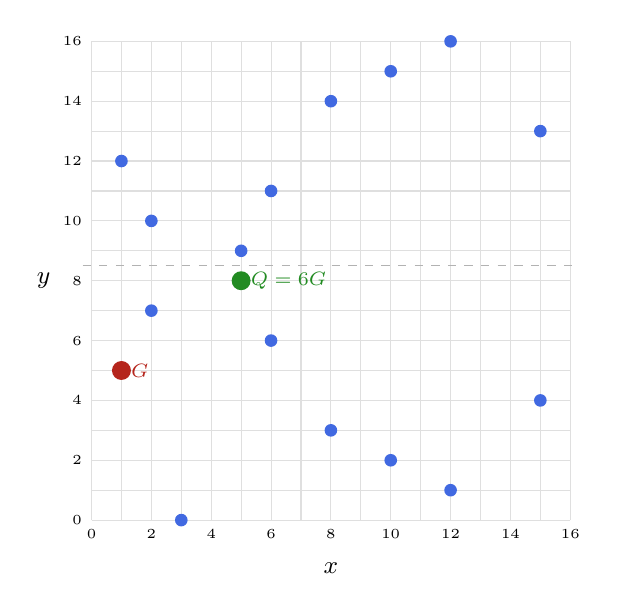
\begin{tikzpicture}[scale=0.38]
    \draw[gray!25] (0,0) grid (16,16);
    \foreach \t in {0,2,...,16} {
      \node[font=\tiny, below] at (\t,0) {\t};
      \node[font=\tiny, left] at (0,\t) {\t};
    }
    \draw[gray!60, dashed] (-0.3,8.5) -- (16.3,8.5);
    \foreach \x/\y in {1/12,2/7,2/10,3/0,5/9,6/6,6/11,8/3,8/14,10/2,10/15,12/1,12/16,15/4,15/13} {
      \fill[RoyalBlue] (\x,\y) circle (6pt);
    }
    \fill[BrickRed] (1,5) circle (9pt) node[right, font=\scriptsize] {$G$};
    \fill[ForestGreen] (5,8) circle (9pt) node[right, font=\scriptsize] {$Q = 6G$};
    \node[font=\small] at (8,-1.6) {$x$};
    \node[font=\small] at (-1.6,8) {$y$};
  \end{tikzpicture}
  \caption{The 17 affine points of $y^2 \equiv x^3 + 7 \pmod{17}$. The set is symmetric with respect to the line $y = 8.5$, because $-y \equiv 17 - y$.}
  \label{fig:toycurve}
\end{figure}

\begin{center}
  \begin{tabular}{l c}
    \toprule
    Points & Order \\
    \midrule
    $(3,0)$ & 2 \\
    $(5,8), (5,9)$ & 3 \\
    $(8,3), (8,14)$ & 6 \\
    $(1,5), (1,12), (2,7), (2,10), (12,1), (12,16)$ & 9 \\
    $(6,6), (6,11), (10,2), (10,15), (15,4), (15,13)$ & 18 \\
    \bottomrule
  \end{tabular}
\end{center}

All orders divide 18, as Lagrange says. The group is cyclic (there are points of order 18, e.g. $(6,6)$, which generate the whole curve), while our base point $G = (1,5)$ has order $9$ and generates only a subgroup of 9 elements.
